\documentclass[twoside]{book}

% Packages required by doxygen
\usepackage{fixltx2e}
\usepackage{calc}
\usepackage{doxygen}
\usepackage[export]{adjustbox} % also loads graphicx
\usepackage{graphicx}
\usepackage[utf8]{inputenc}
\usepackage{makeidx}
\usepackage{multicol}
\usepackage{multirow}
\PassOptionsToPackage{warn}{textcomp}
\usepackage{textcomp}
\usepackage[nointegrals]{wasysym}
\usepackage[table]{xcolor}

% Font selection
\usepackage[T1]{fontenc}
\usepackage[scaled=.90]{helvet}
\usepackage{courier}
\usepackage{amssymb}
\usepackage{sectsty}
\renewcommand{\familydefault}{\sfdefault}
\allsectionsfont{%
  \fontseries{bc}\selectfont%
  \color{darkgray}%
}
\renewcommand{\DoxyLabelFont}{%
  \fontseries{bc}\selectfont%
  \color{darkgray}%
}
\newcommand{\+}{\discretionary{\mbox{\scriptsize$\hookleftarrow$}}{}{}}

% Page & text layout
\usepackage{geometry}
\geometry{%
  a4paper,%
  top=2.5cm,%
  bottom=2.5cm,%
  left=2.5cm,%
  right=2.5cm%
}
\tolerance=750
\hfuzz=15pt
\hbadness=750
\setlength{\emergencystretch}{15pt}
\setlength{\parindent}{0cm}
\setlength{\parskip}{3ex plus 2ex minus 2ex}
\makeatletter
\renewcommand{\paragraph}{%
  \@startsection{paragraph}{4}{0ex}{-1.0ex}{1.0ex}{%
    \normalfont\normalsize\bfseries\SS@parafont%
  }%
}
\renewcommand{\subparagraph}{%
  \@startsection{subparagraph}{5}{0ex}{-1.0ex}{1.0ex}{%
    \normalfont\normalsize\bfseries\SS@subparafont%
  }%
}
\makeatother

% Headers & footers
\usepackage{fancyhdr}
\pagestyle{fancyplain}
\fancyhead[LE]{\fancyplain{}{\bfseries\thepage}}
\fancyhead[CE]{\fancyplain{}{}}
\fancyhead[RE]{\fancyplain{}{\bfseries\leftmark}}
\fancyhead[LO]{\fancyplain{}{\bfseries\rightmark}}
\fancyhead[CO]{\fancyplain{}{}}
\fancyhead[RO]{\fancyplain{}{\bfseries\thepage}}
\fancyfoot[LE]{\fancyplain{}{}}
\fancyfoot[CE]{\fancyplain{}{}}
\fancyfoot[RE]{\fancyplain{}{\bfseries\scriptsize Generated by Doxygen }}
\fancyfoot[LO]{\fancyplain{}{\bfseries\scriptsize Generated by Doxygen }}
\fancyfoot[CO]{\fancyplain{}{}}
\fancyfoot[RO]{\fancyplain{}{}}
\renewcommand{\footrulewidth}{0.4pt}
\renewcommand{\chaptermark}[1]{%
  \markboth{#1}{}%
}
\renewcommand{\sectionmark}[1]{%
  \markright{\thesection\ #1}%
}

% Indices & bibliography
\usepackage{natbib}
\usepackage[titles]{tocloft}
\setcounter{tocdepth}{3}
\setcounter{secnumdepth}{5}
\makeindex

% Hyperlinks (required, but should be loaded last)
\usepackage{ifpdf}
\ifpdf
  \usepackage[pdftex,pagebackref=true]{hyperref}
\else
  \usepackage[ps2pdf,pagebackref=true]{hyperref}
\fi
\hypersetup{%
  colorlinks=true,%
  linkcolor=blue,%
  citecolor=blue,%
  unicode%
}

% Custom commands
\newcommand{\clearemptydoublepage}{%
  \newpage{\pagestyle{empty}\cleardoublepage}%
}

\usepackage{caption}
\captionsetup{labelsep=space,justification=centering,font={bf},singlelinecheck=off,skip=4pt,position=top}

%===== C O N T E N T S =====

\begin{document}

% Titlepage & ToC
\hypersetup{pageanchor=false,
             bookmarksnumbered=true,
             pdfencoding=unicode
            }
\pagenumbering{alph}
\begin{titlepage}
\vspace*{7cm}
\begin{center}%
{\Large Calculator }\\
\vspace*{1cm}
{\large Generated by Doxygen 1.8.14}\\
\end{center}
\end{titlepage}
\clearemptydoublepage
\pagenumbering{roman}
\tableofcontents
\clearemptydoublepage
\pagenumbering{arabic}
\hypersetup{pageanchor=true}

%--- Begin generated contents ---
\chapter{Namespace Index}
\section{Namespace List}
Here is a list of all namespaces with brief descriptions\+:\begin{DoxyCompactList}
\item\contentsline{section}{\mbox{\hyperlink{namespace_p_a_c4_______calculadora}{P\+A\+C4\+\_\+\+\_\+\+\_\+\+Calculadora}} }{\pageref{namespace_p_a_c4_______calculadora}}{}
\end{DoxyCompactList}

\chapter{Hierarchical Index}
\section{Class Hierarchy}
This inheritance list is sorted roughly, but not completely, alphabetically\+:\begin{DoxyCompactList}
\item Window\begin{DoxyCompactList}
\item \contentsline{section}{P\+A\+C4\+\_\+\+\_\+\+\_\+\+Calculadora.\+Main\+Window}{\pageref{class_p_a_c4_______calculadora_1_1_main_window}}{}
\end{DoxyCompactList}
\end{DoxyCompactList}

\chapter{Class Index}
\section{Class List}
Here are the classes, structs, unions and interfaces with brief descriptions\+:\begin{DoxyCompactList}
\item\contentsline{section}{\mbox{\hyperlink{class_p_a_c4_______calculadora_1_1_main_window}{P\+A\+C4\+\_\+\+\_\+\+\_\+\+Calculadora.\+Main\+Window}} \\*This is the \mbox{\hyperlink{class_p_a_c4_______calculadora_1_1_main_window}{Main\+Window}} of the Calculator. }{\pageref{class_p_a_c4_______calculadora_1_1_main_window}}{}
\end{DoxyCompactList}

\chapter{File Index}
\section{File List}
Here is a list of all files with brief descriptions\+:\begin{DoxyCompactList}
\item\contentsline{section}{P\+A\+C4 -\/ Calculadora/\mbox{\hyperlink{_main_window_8xaml_8cs}{Main\+Window.\+xaml.\+cs}} }{\pageref{_main_window_8xaml_8cs}}{}
\end{DoxyCompactList}

\chapter{Namespace Documentation}
\hypertarget{namespace_p_a_c4_______calculadora}{}\section{P\+A\+C4\+\_\+\+\_\+\+\_\+\+Calculadora Namespace Reference}
\label{namespace_p_a_c4_______calculadora}\index{P\+A\+C4\+\_\+\+\_\+\+\_\+\+Calculadora@{P\+A\+C4\+\_\+\+\_\+\+\_\+\+Calculadora}}
\subsection*{Classes}
\begin{DoxyCompactItemize}
\item 
class \mbox{\hyperlink{class_p_a_c4_______calculadora_1_1_main_window}{Main\+Window}}
\begin{DoxyCompactList}\small\item\em This is the \mbox{\hyperlink{class_p_a_c4_______calculadora_1_1_main_window}{Main\+Window}} of the Calculator. \end{DoxyCompactList}\end{DoxyCompactItemize}

\chapter{Class Documentation}
\hypertarget{class_p_a_c4_______calculadora_1_1_main_window}{}\section{P\+A\+C4\+\_\+\+\_\+\+\_\+\+Calculadora.\+Main\+Window Class Reference}
\label{class_p_a_c4_______calculadora_1_1_main_window}\index{P\+A\+C4\+\_\+\+\_\+\+\_\+\+Calculadora.\+Main\+Window@{P\+A\+C4\+\_\+\+\_\+\+\_\+\+Calculadora.\+Main\+Window}}


This is the \mbox{\hyperlink{class_p_a_c4_______calculadora_1_1_main_window}{Main\+Window}} of the Calculator.  


Inheritance diagram for P\+A\+C4\+\_\+\+\_\+\+\_\+\+Calculadora.\+Main\+Window\+:\begin{figure}[H]
\begin{center}
\leavevmode
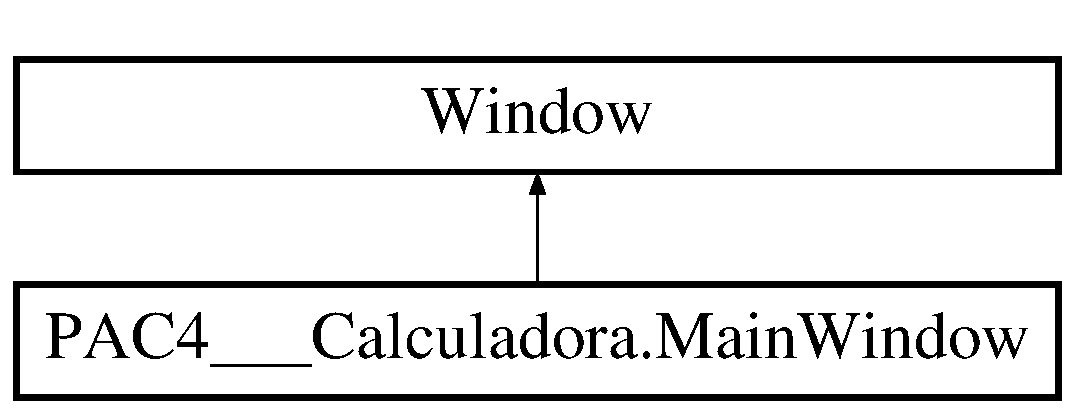
\includegraphics[height=2.000000cm]{class_p_a_c4_______calculadora_1_1_main_window}
\end{center}
\end{figure}
\subsection*{Public Member Functions}
\begin{DoxyCompactItemize}
\item 
\mbox{\hyperlink{class_p_a_c4_______calculadora_1_1_main_window_a3c32f82d8171e5b7b00a5d78c1caad05}{Main\+Window}} ()
\end{DoxyCompactItemize}
\subsection*{Private Member Functions}
\begin{DoxyCompactItemize}
\item 
void \mbox{\hyperlink{class_p_a_c4_______calculadora_1_1_main_window_a735514cee2ee8d58f89d9b2f8d9d49f1}{B\+T\+One\+\_\+\+Click}} (object sender, Routed\+Event\+Args e)
\begin{DoxyCompactList}\small\item\em The logic of the Button 1. It places a 1 in the calculator screen. \end{DoxyCompactList}\item 
void \mbox{\hyperlink{class_p_a_c4_______calculadora_1_1_main_window_a3415f36851e68edf5322a836d57f4d22}{B\+T\+Two\+\_\+\+Click}} (object sender, Routed\+Event\+Args e)
\begin{DoxyCompactList}\small\item\em The logic of the Button 2. It places a 2 in the calculator screen. \end{DoxyCompactList}\item 
void \mbox{\hyperlink{class_p_a_c4_______calculadora_1_1_main_window_a8f8aa1b9eac466368afb1fedaf388113}{B\+T\+Three\+\_\+\+Click}} (object sender, Routed\+Event\+Args e)
\begin{DoxyCompactList}\small\item\em The logic of the Button 3. It places a 3 in the calculator screen. \end{DoxyCompactList}\item 
void \mbox{\hyperlink{class_p_a_c4_______calculadora_1_1_main_window_ab34ce4e048c77bc5963e10f37f8d2332}{B\+T\+Four\+\_\+\+Click}} (object sender, Routed\+Event\+Args e)
\begin{DoxyCompactList}\small\item\em The logic of the Button 4. It places a 4 in the calculator screen. \end{DoxyCompactList}\item 
void \mbox{\hyperlink{class_p_a_c4_______calculadora_1_1_main_window_a4d6c73da40604b904949848d8c1aa7ec}{B\+T\+Five\+\_\+\+Click}} (object sender, Routed\+Event\+Args e)
\begin{DoxyCompactList}\small\item\em The logic of the Button 5. It places a 5 in the calculator screen. \end{DoxyCompactList}\item 
void \mbox{\hyperlink{class_p_a_c4_______calculadora_1_1_main_window_ad6208374e2b207e68156e38e6e1eb4d1}{B\+T\+Six\+\_\+\+Click}} (object sender, Routed\+Event\+Args e)
\begin{DoxyCompactList}\small\item\em The logic of the Button 6. It places a 6 in the calculator screen. \end{DoxyCompactList}\item 
void \mbox{\hyperlink{class_p_a_c4_______calculadora_1_1_main_window_ac6290da671498c9bc01ecc4deef41972}{B\+T\+Seven\+\_\+\+Click}} (object sender, Routed\+Event\+Args e)
\begin{DoxyCompactList}\small\item\em The logic of the Button 7. It places a 7 in the calculator screen. \end{DoxyCompactList}\item 
void \mbox{\hyperlink{class_p_a_c4_______calculadora_1_1_main_window_a09bee2b6053b481bc0e202277af42890}{B\+T\+Eight\+\_\+\+Click}} (object sender, Routed\+Event\+Args e)
\begin{DoxyCompactList}\small\item\em The logic of the Button 8. It places a 8 in the calculator screen. \end{DoxyCompactList}\item 
void \mbox{\hyperlink{class_p_a_c4_______calculadora_1_1_main_window_af146fbab792e00236730856369d69bcc}{B\+T\+Nine\+\_\+\+Click}} (object sender, Routed\+Event\+Args e)
\begin{DoxyCompactList}\small\item\em The logic of the Button 9. It places a 9 in the calculator screen. \end{DoxyCompactList}\item 
void \mbox{\hyperlink{class_p_a_c4_______calculadora_1_1_main_window_ab862d5f81c38770faacbfa15cede92dc}{B\+T\+Zero\+\_\+\+Click}} (object sender, Routed\+Event\+Args e)
\begin{DoxyCompactList}\small\item\em The logic of the Button 0. It places a 0 in the calculator screen. \end{DoxyCompactList}\item 
void \mbox{\hyperlink{class_p_a_c4_______calculadora_1_1_main_window_af87aaed6d16cab4759642fb55f75a241}{B\+T\+Add\+\_\+\+Click}} (object sender, Routed\+Event\+Args e)
\begin{DoxyCompactList}\small\item\em The logic of the Button +. It places a + in the calculator screen. \end{DoxyCompactList}\item 
void \mbox{\hyperlink{class_p_a_c4_______calculadora_1_1_main_window_ade34438d63aa3adde73f310bb3d17d76}{B\+T\+Sub\+\_\+\+Click}} (object sender, Routed\+Event\+Args e)
\begin{DoxyCompactList}\small\item\em The logic of the Button -\/. It places a -\/ in the calculator screen. \end{DoxyCompactList}\item 
void \mbox{\hyperlink{class_p_a_c4_______calculadora_1_1_main_window_a96f6c37dea4ee95cb9c12a9d0383f258}{B\+T\+Mul\+\_\+\+Click}} (object sender, Routed\+Event\+Args e)
\begin{DoxyCompactList}\small\item\em The logic of the Button $\ast$. It places a $\ast$ in the calculator screen. \end{DoxyCompactList}\item 
void \mbox{\hyperlink{class_p_a_c4_______calculadora_1_1_main_window_ae54986bf1f0aeae9fd7906fd69367088}{B\+T\+Div\+\_\+\+Click}} (object sender, Routed\+Event\+Args e)
\begin{DoxyCompactList}\small\item\em The logic of the Button /. It places a / in the calculator screen. \end{DoxyCompactList}\item 
void \mbox{\hyperlink{class_p_a_c4_______calculadora_1_1_main_window_ac9834bfd83a9c94fdf74966604b9bbcf}{B\+T\+Equal\+\_\+\+Click}} (object sender, Routed\+Event\+Args e)
\begin{DoxyCompactList}\small\item\em The logic of the Button =. Writes the result of the current operation on the screen. \end{DoxyCompactList}\item 
void \mbox{\hyperlink{class_p_a_c4_______calculadora_1_1_main_window_aba0b6892ba944cca1a6fc4bb0b1b35ca}{B\+T\+C\+\_\+\+Click}} (object sender, Routed\+Event\+Args e)
\begin{DoxyCompactList}\small\item\em The logic of the Button C. It deletes all the content of the screen. \end{DoxyCompactList}\item 
void \mbox{\hyperlink{class_p_a_c4_______calculadora_1_1_main_window_a7d2be16992dd5a6df70be40c4d9d0dfd}{Screen\+Text\+Changed}} (object sender, Text\+Changed\+Event\+Args e)
\begin{DoxyCompactList}\small\item\em This function updates the last\+Char variable. This variable is used to check if the last character of the screen is a operator, and if it can be placed on the screen. \end{DoxyCompactList}\item 
void \mbox{\hyperlink{class_p_a_c4_______calculadora_1_1_main_window_a45c2b3e046115db99c9e662f6a002afd}{Window\+\_\+\+Key\+Down}} (object sender, Key\+Event\+Args e)
\begin{DoxyCompactList}\small\item\em This function permits the usage of the Num\+Pad of the keyboard in the aplication. \end{DoxyCompactList}\item 
String \mbox{[}$\,$\mbox{]} \mbox{\hyperlink{class_p_a_c4_______calculadora_1_1_main_window_a2ccd0aeaba2aaf4e1535f2bf6fe43e6c}{Butcher\+Operation}} ()
\begin{DoxyCompactList}\small\item\em This function gets the current text on the screen and it divides the text in values and operators in a Array \end{DoxyCompactList}\item 
String \mbox{\hyperlink{class_p_a_c4_______calculadora_1_1_main_window_a58ba74bda855d9a8ce9425450a703dd6}{Calculate}} (String\mbox{[}$\,$\mbox{]} butchered\+Operation)
\begin{DoxyCompactList}\small\item\em This function does the order of operations. \end{DoxyCompactList}\item 
String \mbox{\hyperlink{class_p_a_c4_______calculadora_1_1_main_window_a563642c8d66bce5c42fb1e283c8daedb}{Operator}} (String a, String b, String o)
\begin{DoxyCompactList}\small\item\em This function does the operation, getting the two values and then the operator to decide what operation needs to be done. \end{DoxyCompactList}\item 
String \mbox{[}$\,$\mbox{]} \mbox{\hyperlink{class_p_a_c4_______calculadora_1_1_main_window_ad6d11764ea168d7bd9535ca468769566}{Resize\+Array}} (String\mbox{[}$\,$\mbox{]} butchered\+Operation)
\begin{DoxyCompactList}\small\item\em This function resize the Array to be able to continue with the operations. \end{DoxyCompactList}\end{DoxyCompactItemize}
\subsection*{Private Attributes}
\begin{DoxyCompactItemize}
\item 
String \mbox{\hyperlink{class_p_a_c4_______calculadora_1_1_main_window_aee69de38aec96054ba9ea9b83b202d2d}{Screen\+Text}}
\item 
String \mbox{\hyperlink{class_p_a_c4_______calculadora_1_1_main_window_a4c5f3600067730fbb48d6c7c5d2c8912}{last\+Char}}
\end{DoxyCompactItemize}


\subsection{Detailed Description}
This is the \mbox{\hyperlink{class_p_a_c4_______calculadora_1_1_main_window}{Main\+Window}} of the Calculator. 



\subsection{Constructor \& Destructor Documentation}
\mbox{\Hypertarget{class_p_a_c4_______calculadora_1_1_main_window_a3c32f82d8171e5b7b00a5d78c1caad05}\label{class_p_a_c4_______calculadora_1_1_main_window_a3c32f82d8171e5b7b00a5d78c1caad05}} 
\index{P\+A\+C4\+\_\+\+\_\+\+\_\+\+Calculadora\+::\+Main\+Window@{P\+A\+C4\+\_\+\+\_\+\+\_\+\+Calculadora\+::\+Main\+Window}!Main\+Window@{Main\+Window}}
\index{Main\+Window@{Main\+Window}!P\+A\+C4\+\_\+\+\_\+\+\_\+\+Calculadora\+::\+Main\+Window@{P\+A\+C4\+\_\+\+\_\+\+\_\+\+Calculadora\+::\+Main\+Window}}
\subsubsection{\texorpdfstring{Main\+Window()}{MainWindow()}}
{\footnotesize\ttfamily P\+A\+C4\+\_\+\+\_\+\+\_\+\+Calculadora.\+Main\+Window.\+Main\+Window (\begin{DoxyParamCaption}{ }\end{DoxyParamCaption})\hspace{0.3cm}{\ttfamily [inline]}}



\subsection{Member Function Documentation}
\mbox{\Hypertarget{class_p_a_c4_______calculadora_1_1_main_window_af87aaed6d16cab4759642fb55f75a241}\label{class_p_a_c4_______calculadora_1_1_main_window_af87aaed6d16cab4759642fb55f75a241}} 
\index{P\+A\+C4\+\_\+\+\_\+\+\_\+\+Calculadora\+::\+Main\+Window@{P\+A\+C4\+\_\+\+\_\+\+\_\+\+Calculadora\+::\+Main\+Window}!B\+T\+Add\+\_\+\+Click@{B\+T\+Add\+\_\+\+Click}}
\index{B\+T\+Add\+\_\+\+Click@{B\+T\+Add\+\_\+\+Click}!P\+A\+C4\+\_\+\+\_\+\+\_\+\+Calculadora\+::\+Main\+Window@{P\+A\+C4\+\_\+\+\_\+\+\_\+\+Calculadora\+::\+Main\+Window}}
\subsubsection{\texorpdfstring{B\+T\+Add\+\_\+\+Click()}{BTAdd\_Click()}}
{\footnotesize\ttfamily void P\+A\+C4\+\_\+\+\_\+\+\_\+\+Calculadora.\+Main\+Window.\+B\+T\+Add\+\_\+\+Click (\begin{DoxyParamCaption}\item[{object}]{sender,  }\item[{Routed\+Event\+Args}]{e }\end{DoxyParamCaption})\hspace{0.3cm}{\ttfamily [inline]}, {\ttfamily [private]}}



The logic of the Button +. It places a + in the calculator screen. 

\mbox{\Hypertarget{class_p_a_c4_______calculadora_1_1_main_window_aba0b6892ba944cca1a6fc4bb0b1b35ca}\label{class_p_a_c4_______calculadora_1_1_main_window_aba0b6892ba944cca1a6fc4bb0b1b35ca}} 
\index{P\+A\+C4\+\_\+\+\_\+\+\_\+\+Calculadora\+::\+Main\+Window@{P\+A\+C4\+\_\+\+\_\+\+\_\+\+Calculadora\+::\+Main\+Window}!B\+T\+C\+\_\+\+Click@{B\+T\+C\+\_\+\+Click}}
\index{B\+T\+C\+\_\+\+Click@{B\+T\+C\+\_\+\+Click}!P\+A\+C4\+\_\+\+\_\+\+\_\+\+Calculadora\+::\+Main\+Window@{P\+A\+C4\+\_\+\+\_\+\+\_\+\+Calculadora\+::\+Main\+Window}}
\subsubsection{\texorpdfstring{B\+T\+C\+\_\+\+Click()}{BTC\_Click()}}
{\footnotesize\ttfamily void P\+A\+C4\+\_\+\+\_\+\+\_\+\+Calculadora.\+Main\+Window.\+B\+T\+C\+\_\+\+Click (\begin{DoxyParamCaption}\item[{object}]{sender,  }\item[{Routed\+Event\+Args}]{e }\end{DoxyParamCaption})\hspace{0.3cm}{\ttfamily [inline]}, {\ttfamily [private]}}



The logic of the Button C. It deletes all the content of the screen. 

\mbox{\Hypertarget{class_p_a_c4_______calculadora_1_1_main_window_ae54986bf1f0aeae9fd7906fd69367088}\label{class_p_a_c4_______calculadora_1_1_main_window_ae54986bf1f0aeae9fd7906fd69367088}} 
\index{P\+A\+C4\+\_\+\+\_\+\+\_\+\+Calculadora\+::\+Main\+Window@{P\+A\+C4\+\_\+\+\_\+\+\_\+\+Calculadora\+::\+Main\+Window}!B\+T\+Div\+\_\+\+Click@{B\+T\+Div\+\_\+\+Click}}
\index{B\+T\+Div\+\_\+\+Click@{B\+T\+Div\+\_\+\+Click}!P\+A\+C4\+\_\+\+\_\+\+\_\+\+Calculadora\+::\+Main\+Window@{P\+A\+C4\+\_\+\+\_\+\+\_\+\+Calculadora\+::\+Main\+Window}}
\subsubsection{\texorpdfstring{B\+T\+Div\+\_\+\+Click()}{BTDiv\_Click()}}
{\footnotesize\ttfamily void P\+A\+C4\+\_\+\+\_\+\+\_\+\+Calculadora.\+Main\+Window.\+B\+T\+Div\+\_\+\+Click (\begin{DoxyParamCaption}\item[{object}]{sender,  }\item[{Routed\+Event\+Args}]{e }\end{DoxyParamCaption})\hspace{0.3cm}{\ttfamily [inline]}, {\ttfamily [private]}}



The logic of the Button /. It places a / in the calculator screen. 

\mbox{\Hypertarget{class_p_a_c4_______calculadora_1_1_main_window_a09bee2b6053b481bc0e202277af42890}\label{class_p_a_c4_______calculadora_1_1_main_window_a09bee2b6053b481bc0e202277af42890}} 
\index{P\+A\+C4\+\_\+\+\_\+\+\_\+\+Calculadora\+::\+Main\+Window@{P\+A\+C4\+\_\+\+\_\+\+\_\+\+Calculadora\+::\+Main\+Window}!B\+T\+Eight\+\_\+\+Click@{B\+T\+Eight\+\_\+\+Click}}
\index{B\+T\+Eight\+\_\+\+Click@{B\+T\+Eight\+\_\+\+Click}!P\+A\+C4\+\_\+\+\_\+\+\_\+\+Calculadora\+::\+Main\+Window@{P\+A\+C4\+\_\+\+\_\+\+\_\+\+Calculadora\+::\+Main\+Window}}
\subsubsection{\texorpdfstring{B\+T\+Eight\+\_\+\+Click()}{BTEight\_Click()}}
{\footnotesize\ttfamily void P\+A\+C4\+\_\+\+\_\+\+\_\+\+Calculadora.\+Main\+Window.\+B\+T\+Eight\+\_\+\+Click (\begin{DoxyParamCaption}\item[{object}]{sender,  }\item[{Routed\+Event\+Args}]{e }\end{DoxyParamCaption})\hspace{0.3cm}{\ttfamily [inline]}, {\ttfamily [private]}}



The logic of the Button 8. It places a 8 in the calculator screen. 

\mbox{\Hypertarget{class_p_a_c4_______calculadora_1_1_main_window_ac9834bfd83a9c94fdf74966604b9bbcf}\label{class_p_a_c4_______calculadora_1_1_main_window_ac9834bfd83a9c94fdf74966604b9bbcf}} 
\index{P\+A\+C4\+\_\+\+\_\+\+\_\+\+Calculadora\+::\+Main\+Window@{P\+A\+C4\+\_\+\+\_\+\+\_\+\+Calculadora\+::\+Main\+Window}!B\+T\+Equal\+\_\+\+Click@{B\+T\+Equal\+\_\+\+Click}}
\index{B\+T\+Equal\+\_\+\+Click@{B\+T\+Equal\+\_\+\+Click}!P\+A\+C4\+\_\+\+\_\+\+\_\+\+Calculadora\+::\+Main\+Window@{P\+A\+C4\+\_\+\+\_\+\+\_\+\+Calculadora\+::\+Main\+Window}}
\subsubsection{\texorpdfstring{B\+T\+Equal\+\_\+\+Click()}{BTEqual\_Click()}}
{\footnotesize\ttfamily void P\+A\+C4\+\_\+\+\_\+\+\_\+\+Calculadora.\+Main\+Window.\+B\+T\+Equal\+\_\+\+Click (\begin{DoxyParamCaption}\item[{object}]{sender,  }\item[{Routed\+Event\+Args}]{e }\end{DoxyParamCaption})\hspace{0.3cm}{\ttfamily [inline]}, {\ttfamily [private]}}



The logic of the Button =. Writes the result of the current operation on the screen. 

\mbox{\Hypertarget{class_p_a_c4_______calculadora_1_1_main_window_a4d6c73da40604b904949848d8c1aa7ec}\label{class_p_a_c4_______calculadora_1_1_main_window_a4d6c73da40604b904949848d8c1aa7ec}} 
\index{P\+A\+C4\+\_\+\+\_\+\+\_\+\+Calculadora\+::\+Main\+Window@{P\+A\+C4\+\_\+\+\_\+\+\_\+\+Calculadora\+::\+Main\+Window}!B\+T\+Five\+\_\+\+Click@{B\+T\+Five\+\_\+\+Click}}
\index{B\+T\+Five\+\_\+\+Click@{B\+T\+Five\+\_\+\+Click}!P\+A\+C4\+\_\+\+\_\+\+\_\+\+Calculadora\+::\+Main\+Window@{P\+A\+C4\+\_\+\+\_\+\+\_\+\+Calculadora\+::\+Main\+Window}}
\subsubsection{\texorpdfstring{B\+T\+Five\+\_\+\+Click()}{BTFive\_Click()}}
{\footnotesize\ttfamily void P\+A\+C4\+\_\+\+\_\+\+\_\+\+Calculadora.\+Main\+Window.\+B\+T\+Five\+\_\+\+Click (\begin{DoxyParamCaption}\item[{object}]{sender,  }\item[{Routed\+Event\+Args}]{e }\end{DoxyParamCaption})\hspace{0.3cm}{\ttfamily [inline]}, {\ttfamily [private]}}



The logic of the Button 5. It places a 5 in the calculator screen. 

\mbox{\Hypertarget{class_p_a_c4_______calculadora_1_1_main_window_ab34ce4e048c77bc5963e10f37f8d2332}\label{class_p_a_c4_______calculadora_1_1_main_window_ab34ce4e048c77bc5963e10f37f8d2332}} 
\index{P\+A\+C4\+\_\+\+\_\+\+\_\+\+Calculadora\+::\+Main\+Window@{P\+A\+C4\+\_\+\+\_\+\+\_\+\+Calculadora\+::\+Main\+Window}!B\+T\+Four\+\_\+\+Click@{B\+T\+Four\+\_\+\+Click}}
\index{B\+T\+Four\+\_\+\+Click@{B\+T\+Four\+\_\+\+Click}!P\+A\+C4\+\_\+\+\_\+\+\_\+\+Calculadora\+::\+Main\+Window@{P\+A\+C4\+\_\+\+\_\+\+\_\+\+Calculadora\+::\+Main\+Window}}
\subsubsection{\texorpdfstring{B\+T\+Four\+\_\+\+Click()}{BTFour\_Click()}}
{\footnotesize\ttfamily void P\+A\+C4\+\_\+\+\_\+\+\_\+\+Calculadora.\+Main\+Window.\+B\+T\+Four\+\_\+\+Click (\begin{DoxyParamCaption}\item[{object}]{sender,  }\item[{Routed\+Event\+Args}]{e }\end{DoxyParamCaption})\hspace{0.3cm}{\ttfamily [inline]}, {\ttfamily [private]}}



The logic of the Button 4. It places a 4 in the calculator screen. 

\mbox{\Hypertarget{class_p_a_c4_______calculadora_1_1_main_window_a96f6c37dea4ee95cb9c12a9d0383f258}\label{class_p_a_c4_______calculadora_1_1_main_window_a96f6c37dea4ee95cb9c12a9d0383f258}} 
\index{P\+A\+C4\+\_\+\+\_\+\+\_\+\+Calculadora\+::\+Main\+Window@{P\+A\+C4\+\_\+\+\_\+\+\_\+\+Calculadora\+::\+Main\+Window}!B\+T\+Mul\+\_\+\+Click@{B\+T\+Mul\+\_\+\+Click}}
\index{B\+T\+Mul\+\_\+\+Click@{B\+T\+Mul\+\_\+\+Click}!P\+A\+C4\+\_\+\+\_\+\+\_\+\+Calculadora\+::\+Main\+Window@{P\+A\+C4\+\_\+\+\_\+\+\_\+\+Calculadora\+::\+Main\+Window}}
\subsubsection{\texorpdfstring{B\+T\+Mul\+\_\+\+Click()}{BTMul\_Click()}}
{\footnotesize\ttfamily void P\+A\+C4\+\_\+\+\_\+\+\_\+\+Calculadora.\+Main\+Window.\+B\+T\+Mul\+\_\+\+Click (\begin{DoxyParamCaption}\item[{object}]{sender,  }\item[{Routed\+Event\+Args}]{e }\end{DoxyParamCaption})\hspace{0.3cm}{\ttfamily [inline]}, {\ttfamily [private]}}



The logic of the Button $\ast$. It places a $\ast$ in the calculator screen. 

\mbox{\Hypertarget{class_p_a_c4_______calculadora_1_1_main_window_af146fbab792e00236730856369d69bcc}\label{class_p_a_c4_______calculadora_1_1_main_window_af146fbab792e00236730856369d69bcc}} 
\index{P\+A\+C4\+\_\+\+\_\+\+\_\+\+Calculadora\+::\+Main\+Window@{P\+A\+C4\+\_\+\+\_\+\+\_\+\+Calculadora\+::\+Main\+Window}!B\+T\+Nine\+\_\+\+Click@{B\+T\+Nine\+\_\+\+Click}}
\index{B\+T\+Nine\+\_\+\+Click@{B\+T\+Nine\+\_\+\+Click}!P\+A\+C4\+\_\+\+\_\+\+\_\+\+Calculadora\+::\+Main\+Window@{P\+A\+C4\+\_\+\+\_\+\+\_\+\+Calculadora\+::\+Main\+Window}}
\subsubsection{\texorpdfstring{B\+T\+Nine\+\_\+\+Click()}{BTNine\_Click()}}
{\footnotesize\ttfamily void P\+A\+C4\+\_\+\+\_\+\+\_\+\+Calculadora.\+Main\+Window.\+B\+T\+Nine\+\_\+\+Click (\begin{DoxyParamCaption}\item[{object}]{sender,  }\item[{Routed\+Event\+Args}]{e }\end{DoxyParamCaption})\hspace{0.3cm}{\ttfamily [inline]}, {\ttfamily [private]}}



The logic of the Button 9. It places a 9 in the calculator screen. 

\mbox{\Hypertarget{class_p_a_c4_______calculadora_1_1_main_window_a735514cee2ee8d58f89d9b2f8d9d49f1}\label{class_p_a_c4_______calculadora_1_1_main_window_a735514cee2ee8d58f89d9b2f8d9d49f1}} 
\index{P\+A\+C4\+\_\+\+\_\+\+\_\+\+Calculadora\+::\+Main\+Window@{P\+A\+C4\+\_\+\+\_\+\+\_\+\+Calculadora\+::\+Main\+Window}!B\+T\+One\+\_\+\+Click@{B\+T\+One\+\_\+\+Click}}
\index{B\+T\+One\+\_\+\+Click@{B\+T\+One\+\_\+\+Click}!P\+A\+C4\+\_\+\+\_\+\+\_\+\+Calculadora\+::\+Main\+Window@{P\+A\+C4\+\_\+\+\_\+\+\_\+\+Calculadora\+::\+Main\+Window}}
\subsubsection{\texorpdfstring{B\+T\+One\+\_\+\+Click()}{BTOne\_Click()}}
{\footnotesize\ttfamily void P\+A\+C4\+\_\+\+\_\+\+\_\+\+Calculadora.\+Main\+Window.\+B\+T\+One\+\_\+\+Click (\begin{DoxyParamCaption}\item[{object}]{sender,  }\item[{Routed\+Event\+Args}]{e }\end{DoxyParamCaption})\hspace{0.3cm}{\ttfamily [inline]}, {\ttfamily [private]}}



The logic of the Button 1. It places a 1 in the calculator screen. 

\mbox{\Hypertarget{class_p_a_c4_______calculadora_1_1_main_window_ac6290da671498c9bc01ecc4deef41972}\label{class_p_a_c4_______calculadora_1_1_main_window_ac6290da671498c9bc01ecc4deef41972}} 
\index{P\+A\+C4\+\_\+\+\_\+\+\_\+\+Calculadora\+::\+Main\+Window@{P\+A\+C4\+\_\+\+\_\+\+\_\+\+Calculadora\+::\+Main\+Window}!B\+T\+Seven\+\_\+\+Click@{B\+T\+Seven\+\_\+\+Click}}
\index{B\+T\+Seven\+\_\+\+Click@{B\+T\+Seven\+\_\+\+Click}!P\+A\+C4\+\_\+\+\_\+\+\_\+\+Calculadora\+::\+Main\+Window@{P\+A\+C4\+\_\+\+\_\+\+\_\+\+Calculadora\+::\+Main\+Window}}
\subsubsection{\texorpdfstring{B\+T\+Seven\+\_\+\+Click()}{BTSeven\_Click()}}
{\footnotesize\ttfamily void P\+A\+C4\+\_\+\+\_\+\+\_\+\+Calculadora.\+Main\+Window.\+B\+T\+Seven\+\_\+\+Click (\begin{DoxyParamCaption}\item[{object}]{sender,  }\item[{Routed\+Event\+Args}]{e }\end{DoxyParamCaption})\hspace{0.3cm}{\ttfamily [inline]}, {\ttfamily [private]}}



The logic of the Button 7. It places a 7 in the calculator screen. 

\mbox{\Hypertarget{class_p_a_c4_______calculadora_1_1_main_window_ad6208374e2b207e68156e38e6e1eb4d1}\label{class_p_a_c4_______calculadora_1_1_main_window_ad6208374e2b207e68156e38e6e1eb4d1}} 
\index{P\+A\+C4\+\_\+\+\_\+\+\_\+\+Calculadora\+::\+Main\+Window@{P\+A\+C4\+\_\+\+\_\+\+\_\+\+Calculadora\+::\+Main\+Window}!B\+T\+Six\+\_\+\+Click@{B\+T\+Six\+\_\+\+Click}}
\index{B\+T\+Six\+\_\+\+Click@{B\+T\+Six\+\_\+\+Click}!P\+A\+C4\+\_\+\+\_\+\+\_\+\+Calculadora\+::\+Main\+Window@{P\+A\+C4\+\_\+\+\_\+\+\_\+\+Calculadora\+::\+Main\+Window}}
\subsubsection{\texorpdfstring{B\+T\+Six\+\_\+\+Click()}{BTSix\_Click()}}
{\footnotesize\ttfamily void P\+A\+C4\+\_\+\+\_\+\+\_\+\+Calculadora.\+Main\+Window.\+B\+T\+Six\+\_\+\+Click (\begin{DoxyParamCaption}\item[{object}]{sender,  }\item[{Routed\+Event\+Args}]{e }\end{DoxyParamCaption})\hspace{0.3cm}{\ttfamily [inline]}, {\ttfamily [private]}}



The logic of the Button 6. It places a 6 in the calculator screen. 

\mbox{\Hypertarget{class_p_a_c4_______calculadora_1_1_main_window_ade34438d63aa3adde73f310bb3d17d76}\label{class_p_a_c4_______calculadora_1_1_main_window_ade34438d63aa3adde73f310bb3d17d76}} 
\index{P\+A\+C4\+\_\+\+\_\+\+\_\+\+Calculadora\+::\+Main\+Window@{P\+A\+C4\+\_\+\+\_\+\+\_\+\+Calculadora\+::\+Main\+Window}!B\+T\+Sub\+\_\+\+Click@{B\+T\+Sub\+\_\+\+Click}}
\index{B\+T\+Sub\+\_\+\+Click@{B\+T\+Sub\+\_\+\+Click}!P\+A\+C4\+\_\+\+\_\+\+\_\+\+Calculadora\+::\+Main\+Window@{P\+A\+C4\+\_\+\+\_\+\+\_\+\+Calculadora\+::\+Main\+Window}}
\subsubsection{\texorpdfstring{B\+T\+Sub\+\_\+\+Click()}{BTSub\_Click()}}
{\footnotesize\ttfamily void P\+A\+C4\+\_\+\+\_\+\+\_\+\+Calculadora.\+Main\+Window.\+B\+T\+Sub\+\_\+\+Click (\begin{DoxyParamCaption}\item[{object}]{sender,  }\item[{Routed\+Event\+Args}]{e }\end{DoxyParamCaption})\hspace{0.3cm}{\ttfamily [inline]}, {\ttfamily [private]}}



The logic of the Button -\/. It places a -\/ in the calculator screen. 

\mbox{\Hypertarget{class_p_a_c4_______calculadora_1_1_main_window_a8f8aa1b9eac466368afb1fedaf388113}\label{class_p_a_c4_______calculadora_1_1_main_window_a8f8aa1b9eac466368afb1fedaf388113}} 
\index{P\+A\+C4\+\_\+\+\_\+\+\_\+\+Calculadora\+::\+Main\+Window@{P\+A\+C4\+\_\+\+\_\+\+\_\+\+Calculadora\+::\+Main\+Window}!B\+T\+Three\+\_\+\+Click@{B\+T\+Three\+\_\+\+Click}}
\index{B\+T\+Three\+\_\+\+Click@{B\+T\+Three\+\_\+\+Click}!P\+A\+C4\+\_\+\+\_\+\+\_\+\+Calculadora\+::\+Main\+Window@{P\+A\+C4\+\_\+\+\_\+\+\_\+\+Calculadora\+::\+Main\+Window}}
\subsubsection{\texorpdfstring{B\+T\+Three\+\_\+\+Click()}{BTThree\_Click()}}
{\footnotesize\ttfamily void P\+A\+C4\+\_\+\+\_\+\+\_\+\+Calculadora.\+Main\+Window.\+B\+T\+Three\+\_\+\+Click (\begin{DoxyParamCaption}\item[{object}]{sender,  }\item[{Routed\+Event\+Args}]{e }\end{DoxyParamCaption})\hspace{0.3cm}{\ttfamily [inline]}, {\ttfamily [private]}}



The logic of the Button 3. It places a 3 in the calculator screen. 

\mbox{\Hypertarget{class_p_a_c4_______calculadora_1_1_main_window_a3415f36851e68edf5322a836d57f4d22}\label{class_p_a_c4_______calculadora_1_1_main_window_a3415f36851e68edf5322a836d57f4d22}} 
\index{P\+A\+C4\+\_\+\+\_\+\+\_\+\+Calculadora\+::\+Main\+Window@{P\+A\+C4\+\_\+\+\_\+\+\_\+\+Calculadora\+::\+Main\+Window}!B\+T\+Two\+\_\+\+Click@{B\+T\+Two\+\_\+\+Click}}
\index{B\+T\+Two\+\_\+\+Click@{B\+T\+Two\+\_\+\+Click}!P\+A\+C4\+\_\+\+\_\+\+\_\+\+Calculadora\+::\+Main\+Window@{P\+A\+C4\+\_\+\+\_\+\+\_\+\+Calculadora\+::\+Main\+Window}}
\subsubsection{\texorpdfstring{B\+T\+Two\+\_\+\+Click()}{BTTwo\_Click()}}
{\footnotesize\ttfamily void P\+A\+C4\+\_\+\+\_\+\+\_\+\+Calculadora.\+Main\+Window.\+B\+T\+Two\+\_\+\+Click (\begin{DoxyParamCaption}\item[{object}]{sender,  }\item[{Routed\+Event\+Args}]{e }\end{DoxyParamCaption})\hspace{0.3cm}{\ttfamily [inline]}, {\ttfamily [private]}}



The logic of the Button 2. It places a 2 in the calculator screen. 

\mbox{\Hypertarget{class_p_a_c4_______calculadora_1_1_main_window_ab862d5f81c38770faacbfa15cede92dc}\label{class_p_a_c4_______calculadora_1_1_main_window_ab862d5f81c38770faacbfa15cede92dc}} 
\index{P\+A\+C4\+\_\+\+\_\+\+\_\+\+Calculadora\+::\+Main\+Window@{P\+A\+C4\+\_\+\+\_\+\+\_\+\+Calculadora\+::\+Main\+Window}!B\+T\+Zero\+\_\+\+Click@{B\+T\+Zero\+\_\+\+Click}}
\index{B\+T\+Zero\+\_\+\+Click@{B\+T\+Zero\+\_\+\+Click}!P\+A\+C4\+\_\+\+\_\+\+\_\+\+Calculadora\+::\+Main\+Window@{P\+A\+C4\+\_\+\+\_\+\+\_\+\+Calculadora\+::\+Main\+Window}}
\subsubsection{\texorpdfstring{B\+T\+Zero\+\_\+\+Click()}{BTZero\_Click()}}
{\footnotesize\ttfamily void P\+A\+C4\+\_\+\+\_\+\+\_\+\+Calculadora.\+Main\+Window.\+B\+T\+Zero\+\_\+\+Click (\begin{DoxyParamCaption}\item[{object}]{sender,  }\item[{Routed\+Event\+Args}]{e }\end{DoxyParamCaption})\hspace{0.3cm}{\ttfamily [inline]}, {\ttfamily [private]}}



The logic of the Button 0. It places a 0 in the calculator screen. 

\mbox{\Hypertarget{class_p_a_c4_______calculadora_1_1_main_window_a2ccd0aeaba2aaf4e1535f2bf6fe43e6c}\label{class_p_a_c4_______calculadora_1_1_main_window_a2ccd0aeaba2aaf4e1535f2bf6fe43e6c}} 
\index{P\+A\+C4\+\_\+\+\_\+\+\_\+\+Calculadora\+::\+Main\+Window@{P\+A\+C4\+\_\+\+\_\+\+\_\+\+Calculadora\+::\+Main\+Window}!Butcher\+Operation@{Butcher\+Operation}}
\index{Butcher\+Operation@{Butcher\+Operation}!P\+A\+C4\+\_\+\+\_\+\+\_\+\+Calculadora\+::\+Main\+Window@{P\+A\+C4\+\_\+\+\_\+\+\_\+\+Calculadora\+::\+Main\+Window}}
\subsubsection{\texorpdfstring{Butcher\+Operation()}{ButcherOperation()}}
{\footnotesize\ttfamily String \mbox{[}$\,$\mbox{]} P\+A\+C4\+\_\+\+\_\+\+\_\+\+Calculadora.\+Main\+Window.\+Butcher\+Operation (\begin{DoxyParamCaption}{ }\end{DoxyParamCaption})\hspace{0.3cm}{\ttfamily [inline]}, {\ttfamily [private]}}



This function gets the current text on the screen and it divides the text in values and operators in a Array 

\begin{DoxyReturn}{Returns}
String\mbox{[}\mbox{]} of the values and operators of the screen text
\end{DoxyReturn}
\mbox{\Hypertarget{class_p_a_c4_______calculadora_1_1_main_window_a58ba74bda855d9a8ce9425450a703dd6}\label{class_p_a_c4_______calculadora_1_1_main_window_a58ba74bda855d9a8ce9425450a703dd6}} 
\index{P\+A\+C4\+\_\+\+\_\+\+\_\+\+Calculadora\+::\+Main\+Window@{P\+A\+C4\+\_\+\+\_\+\+\_\+\+Calculadora\+::\+Main\+Window}!Calculate@{Calculate}}
\index{Calculate@{Calculate}!P\+A\+C4\+\_\+\+\_\+\+\_\+\+Calculadora\+::\+Main\+Window@{P\+A\+C4\+\_\+\+\_\+\+\_\+\+Calculadora\+::\+Main\+Window}}
\subsubsection{\texorpdfstring{Calculate()}{Calculate()}}
{\footnotesize\ttfamily String P\+A\+C4\+\_\+\+\_\+\+\_\+\+Calculadora.\+Main\+Window.\+Calculate (\begin{DoxyParamCaption}\item[{String \mbox{[}$\,$\mbox{]}}]{butchered\+Operation }\end{DoxyParamCaption})\hspace{0.3cm}{\ttfamily [inline]}, {\ttfamily [private]}}



This function does the order of operations. 


\begin{DoxyParams}{Parameters}
{\em butchered\+Operation} & The array of values and operators\\
\hline
\end{DoxyParams}
\begin{DoxyReturn}{Returns}
Returns the String final result of the operation.
\end{DoxyReturn}
\mbox{\Hypertarget{class_p_a_c4_______calculadora_1_1_main_window_a563642c8d66bce5c42fb1e283c8daedb}\label{class_p_a_c4_______calculadora_1_1_main_window_a563642c8d66bce5c42fb1e283c8daedb}} 
\index{P\+A\+C4\+\_\+\+\_\+\+\_\+\+Calculadora\+::\+Main\+Window@{P\+A\+C4\+\_\+\+\_\+\+\_\+\+Calculadora\+::\+Main\+Window}!Operator@{Operator}}
\index{Operator@{Operator}!P\+A\+C4\+\_\+\+\_\+\+\_\+\+Calculadora\+::\+Main\+Window@{P\+A\+C4\+\_\+\+\_\+\+\_\+\+Calculadora\+::\+Main\+Window}}
\subsubsection{\texorpdfstring{Operator()}{Operator()}}
{\footnotesize\ttfamily String P\+A\+C4\+\_\+\+\_\+\+\_\+\+Calculadora.\+Main\+Window.\+Operator (\begin{DoxyParamCaption}\item[{String}]{a,  }\item[{String}]{b,  }\item[{String}]{o }\end{DoxyParamCaption})\hspace{0.3cm}{\ttfamily [inline]}, {\ttfamily [private]}}



This function does the operation, getting the two values and then the operator to decide what operation needs to be done. 


\begin{DoxyParams}{Parameters}
{\em a} & The first value\\
\hline
{\em b} & The second value\\
\hline
{\em o} & The operator\\
\hline
\end{DoxyParams}
\begin{DoxyReturn}{Returns}
Returns the String result of the operation. In case you devide for 0 it returns error
\end{DoxyReturn}
\mbox{\Hypertarget{class_p_a_c4_______calculadora_1_1_main_window_ad6d11764ea168d7bd9535ca468769566}\label{class_p_a_c4_______calculadora_1_1_main_window_ad6d11764ea168d7bd9535ca468769566}} 
\index{P\+A\+C4\+\_\+\+\_\+\+\_\+\+Calculadora\+::\+Main\+Window@{P\+A\+C4\+\_\+\+\_\+\+\_\+\+Calculadora\+::\+Main\+Window}!Resize\+Array@{Resize\+Array}}
\index{Resize\+Array@{Resize\+Array}!P\+A\+C4\+\_\+\+\_\+\+\_\+\+Calculadora\+::\+Main\+Window@{P\+A\+C4\+\_\+\+\_\+\+\_\+\+Calculadora\+::\+Main\+Window}}
\subsubsection{\texorpdfstring{Resize\+Array()}{ResizeArray()}}
{\footnotesize\ttfamily String \mbox{[}$\,$\mbox{]} P\+A\+C4\+\_\+\+\_\+\+\_\+\+Calculadora.\+Main\+Window.\+Resize\+Array (\begin{DoxyParamCaption}\item[{String \mbox{[}$\,$\mbox{]}}]{butchered\+Operation }\end{DoxyParamCaption})\hspace{0.3cm}{\ttfamily [inline]}, {\ttfamily [private]}}



This function resize the Array to be able to continue with the operations. 


\begin{DoxyParams}{Parameters}
{\em butchered\+Operation} & The array of values and operators\\
\hline
\end{DoxyParams}
\begin{DoxyReturn}{Returns}
Returns the String\mbox{[}\mbox{]} with the new size
\end{DoxyReturn}
\mbox{\Hypertarget{class_p_a_c4_______calculadora_1_1_main_window_a7d2be16992dd5a6df70be40c4d9d0dfd}\label{class_p_a_c4_______calculadora_1_1_main_window_a7d2be16992dd5a6df70be40c4d9d0dfd}} 
\index{P\+A\+C4\+\_\+\+\_\+\+\_\+\+Calculadora\+::\+Main\+Window@{P\+A\+C4\+\_\+\+\_\+\+\_\+\+Calculadora\+::\+Main\+Window}!Screen\+Text\+Changed@{Screen\+Text\+Changed}}
\index{Screen\+Text\+Changed@{Screen\+Text\+Changed}!P\+A\+C4\+\_\+\+\_\+\+\_\+\+Calculadora\+::\+Main\+Window@{P\+A\+C4\+\_\+\+\_\+\+\_\+\+Calculadora\+::\+Main\+Window}}
\subsubsection{\texorpdfstring{Screen\+Text\+Changed()}{ScreenTextChanged()}}
{\footnotesize\ttfamily void P\+A\+C4\+\_\+\+\_\+\+\_\+\+Calculadora.\+Main\+Window.\+Screen\+Text\+Changed (\begin{DoxyParamCaption}\item[{object}]{sender,  }\item[{Text\+Changed\+Event\+Args}]{e }\end{DoxyParamCaption})\hspace{0.3cm}{\ttfamily [inline]}, {\ttfamily [private]}}



This function updates the last\+Char variable. This variable is used to check if the last character of the screen is a operator, and if it can be placed on the screen. 

\mbox{\Hypertarget{class_p_a_c4_______calculadora_1_1_main_window_a45c2b3e046115db99c9e662f6a002afd}\label{class_p_a_c4_______calculadora_1_1_main_window_a45c2b3e046115db99c9e662f6a002afd}} 
\index{P\+A\+C4\+\_\+\+\_\+\+\_\+\+Calculadora\+::\+Main\+Window@{P\+A\+C4\+\_\+\+\_\+\+\_\+\+Calculadora\+::\+Main\+Window}!Window\+\_\+\+Key\+Down@{Window\+\_\+\+Key\+Down}}
\index{Window\+\_\+\+Key\+Down@{Window\+\_\+\+Key\+Down}!P\+A\+C4\+\_\+\+\_\+\+\_\+\+Calculadora\+::\+Main\+Window@{P\+A\+C4\+\_\+\+\_\+\+\_\+\+Calculadora\+::\+Main\+Window}}
\subsubsection{\texorpdfstring{Window\+\_\+\+Key\+Down()}{Window\_KeyDown()}}
{\footnotesize\ttfamily void P\+A\+C4\+\_\+\+\_\+\+\_\+\+Calculadora.\+Main\+Window.\+Window\+\_\+\+Key\+Down (\begin{DoxyParamCaption}\item[{object}]{sender,  }\item[{Key\+Event\+Args}]{e }\end{DoxyParamCaption})\hspace{0.3cm}{\ttfamily [inline]}, {\ttfamily [private]}}



This function permits the usage of the Num\+Pad of the keyboard in the aplication. 



\subsection{Member Data Documentation}
\mbox{\Hypertarget{class_p_a_c4_______calculadora_1_1_main_window_a4c5f3600067730fbb48d6c7c5d2c8912}\label{class_p_a_c4_______calculadora_1_1_main_window_a4c5f3600067730fbb48d6c7c5d2c8912}} 
\index{P\+A\+C4\+\_\+\+\_\+\+\_\+\+Calculadora\+::\+Main\+Window@{P\+A\+C4\+\_\+\+\_\+\+\_\+\+Calculadora\+::\+Main\+Window}!last\+Char@{last\+Char}}
\index{last\+Char@{last\+Char}!P\+A\+C4\+\_\+\+\_\+\+\_\+\+Calculadora\+::\+Main\+Window@{P\+A\+C4\+\_\+\+\_\+\+\_\+\+Calculadora\+::\+Main\+Window}}
\subsubsection{\texorpdfstring{last\+Char}{lastChar}}
{\footnotesize\ttfamily String P\+A\+C4\+\_\+\+\_\+\+\_\+\+Calculadora.\+Main\+Window.\+last\+Char\hspace{0.3cm}{\ttfamily [private]}}

\mbox{\Hypertarget{class_p_a_c4_______calculadora_1_1_main_window_aee69de38aec96054ba9ea9b83b202d2d}\label{class_p_a_c4_______calculadora_1_1_main_window_aee69de38aec96054ba9ea9b83b202d2d}} 
\index{P\+A\+C4\+\_\+\+\_\+\+\_\+\+Calculadora\+::\+Main\+Window@{P\+A\+C4\+\_\+\+\_\+\+\_\+\+Calculadora\+::\+Main\+Window}!Screen\+Text@{Screen\+Text}}
\index{Screen\+Text@{Screen\+Text}!P\+A\+C4\+\_\+\+\_\+\+\_\+\+Calculadora\+::\+Main\+Window@{P\+A\+C4\+\_\+\+\_\+\+\_\+\+Calculadora\+::\+Main\+Window}}
\subsubsection{\texorpdfstring{Screen\+Text}{ScreenText}}
{\footnotesize\ttfamily String P\+A\+C4\+\_\+\+\_\+\+\_\+\+Calculadora.\+Main\+Window.\+Screen\+Text\hspace{0.3cm}{\ttfamily [private]}}



The documentation for this class was generated from the following file\+:\begin{DoxyCompactItemize}
\item 
P\+A\+C4 -\/ Calculadora/\mbox{\hyperlink{_main_window_8xaml_8cs}{Main\+Window.\+xaml.\+cs}}\end{DoxyCompactItemize}

\chapter{File Documentation}
\hypertarget{_main_window_8xaml_8cs}{}\section{P\+A\+C4 -\/ Calculadora/\+Main\+Window.xaml.\+cs File Reference}
\label{_main_window_8xaml_8cs}\index{P\+A\+C4 -\/ Calculadora/\+Main\+Window.\+xaml.\+cs@{P\+A\+C4 -\/ Calculadora/\+Main\+Window.\+xaml.\+cs}}
\subsection*{Classes}
\begin{DoxyCompactItemize}
\item 
class \mbox{\hyperlink{class_p_a_c4_______calculadora_1_1_main_window}{P\+A\+C4\+\_\+\+\_\+\+\_\+\+Calculadora.\+Main\+Window}}
\begin{DoxyCompactList}\small\item\em This is the \mbox{\hyperlink{class_p_a_c4_______calculadora_1_1_main_window}{Main\+Window}} of the Calculator. \end{DoxyCompactList}\end{DoxyCompactItemize}
\subsection*{Namespaces}
\begin{DoxyCompactItemize}
\item 
namespace \mbox{\hyperlink{namespace_p_a_c4_______calculadora}{P\+A\+C4\+\_\+\+\_\+\+\_\+\+Calculadora}}
\end{DoxyCompactItemize}

%--- End generated contents ---

% Index
\backmatter
\newpage
\phantomsection
\clearemptydoublepage
\addcontentsline{toc}{chapter}{Index}
\printindex

\end{document}
